This chapter presents the proposed concept for verifying AI-generated DeFi
requests before blockchain execution. The concept describes the solution at an
abstract and implementation-independent level. It defines the responsibilities
of the main components, the information exchanged between them, and their
intended behaviour without prescribing a specific programming language,
database system, query language, wallet implementation, or software framework.

The concept follows from the findings of the State of the Art in
Chapter~\ref{chap:stateoftheart}. The analysis showed that the investigated
approaches address different parts of the AI-to-blockchain execution problem.
AI-agent blockchain execution approaches provide mechanisms for interpreting
natural-language requests and transforming them into structured actions.
Knowledge retrieval and grounding approaches contribute external and updateable
information. Graph-based approaches provide an explicit representation of DeFi
entities and their relationships, while execution-layer security approaches
provide mechanisms for restricting blockchain execution. None of these
approach groups alone provides the complete workflow required by the
requirements defined in Section~\ref{sec:requirements_analysis}. The proposed
concept therefore combines complementary characteristics of these approaches.

The proposed solution separates natural-language interpretation, deterministic
intent validation, authoritative relationship verification, and controlled
blockchain execution. A language model first generates a candidate structured
intent. Deterministic checks establish whether this intent is suitable for
verification. The validated intent is then evaluated against authoritative
graph-based verification knowledge. Only a successfully verified operation is
allowed to continue toward controlled smart-wallet execution.



% =========================================================
% 3.1 Overall System Concept
% =========================================================

\section{Overall System Concept}
\label{sec:overall_system_concept}

The proposed system introduces a mandatory verification boundary between the
interpretation of a user's DeFi request and blockchain execution. This boundary
is necessary because individually valid blockchain entities do not necessarily
form a valid execution combination. A protocol, contract, callable function,
asset, pool, or reserve may each be legitimate independently while still being
incorrectly combined for a particular action, protocol deployment, or
blockchain network.

The proposed concept combines complementary capabilities identified in the
chapter~\ref{chap:stateoftheart}. AI-agent approaches provide natural-language interpretation,
knowledge-retrieval approaches contribute external and updateable protocol
information, graph-based approaches provide explicit representation of DeFi
entities and their relationships, and execution-layer approaches provide
mechanisms for restricting blockchain execution. The proposed system combines
these capabilities into a pre-execution verification workflow rather than
attempting to replace them.

As illustrated in Figure~\ref{fig:system_architecture}, the proposed system
is organized into four architectural subsystems: AI/Intent, Verification
Knowledge, Relationship Verification, and Controlled Execution. Together,
these subsystems provide five main conceptual elements:

\begin{enumerate}

    \item \textbf{LLM-Based Intent Generation} interprets the user's
    natural-language request and transforms it into a machine-readable
    candidate intent describing the requested DeFi operation. The language
    model identifies what the user intends to perform but does not determine
    the complete blockchain execution path.

    \item \textbf{Intent Validation} checks whether the candidate intent is
    sufficiently complete, valid, supported, and unambiguous for subsequent
    verification. Invalid or unresolved intents are not allowed to proceed.

    \item \textbf{Authoritative Verification Knowledge} provides the trusted
    reference used during verification. It represents accepted information
    about protocol deployments, supported actions, contracts, functions,
    assets, pools, reserves, and their relationships as a maintained
    graph-based knowledge model.

    \item \textbf{Relationship Verification and Decision} evaluates the
    validated intent against the authoritative verification knowledge. It returns approval when the required relationships are established, rejection when the evidence rules them out, and verification failure when the evidence is insufficient for either conclusion.

\item \textbf{Controlled Smart-Wallet Execution} receives an approved
verification result and checks its validity before blockchain submission.
Execution is permitted only if the protected parameters remain unchanged,
the approval has not expired, and the referenced verification evidence
remains applicable. Otherwise, the operation must be verified again.

\end{enumerate}

The five elements do not form a purely sequential pipeline.
\textbf{Authoritative Verification Knowledge} is maintained independently and
acts as a supporting knowledge source for
\textbf{Relationship Verification and Decision}. The request-processing path
therefore proceeds from intent generation to intent validation, relationship
verification, and controlled execution, while verification knowledge is
acquired and maintained separately.

Figure~\ref{fig:overall_system_flow} illustrates how an individual DeFi
request is processed from natural-language input to controlled smart-wallet
    execution. 

\begin{figure}[H]
    \centering
    \resizebox{0.90\textwidth}{!}{%
        % % % =========================================================
% % % overall_system_flow
% % % =========================================================

% \begingroup
% \hyphenpenalty=10000
% \exhyphenpenalty=10000
% \begin{tikzpicture}[x=1cm,y=1cm,>=stealth]
% \path[use as bounding box] (0,0.45) rectangle (16.00,22.55);

% % Subsystem colours, consistent with the component diagram.
% \definecolor{archline}{HTML}{26384C}
% \definecolor{aiborder}{HTML}{1261A8}
% \definecolor{aifill}{HTML}{DCEBFE}
% \definecolor{verborder}{HTML}{6842B5}
% \definecolor{verfill}{HTML}{E9DDFB}
% \definecolor{knowborder}{HTML}{338A49}
% \definecolor{knowfill}{HTML}{DDF3DF}
% \definecolor{execborder}{HTML}{B97800}
% \definecolor{execfill}{HTML}{FCE8B8}
% \definecolor{extborder}{HTML}{5B6677}
% \definecolor{extfill}{HTML}{E4E6EA}

% \tikzset{
%   flowbox/.style={rectangle,rounded corners=3pt,line width=0.7pt,
%     align=center,text=archline,font=\sffamily\fontsize{9.3}{11.2}\selectfont,
%     text width=4.30cm,minimum width=4.80cm,minimum height=1.05cm,
%     inner xsep=3pt,inner ysep=3pt,outer sep=0pt},
%   ai/.style={flowbox,draw=aiborder,fill=aifill},
%   verification/.style={flowbox,draw=verborder,fill=verfill},
%   execution/.style={flowbox,draw=execborder,fill=execfill},
%   external/.style={flowbox,draw=extborder,fill=extfill},
%   knowledge/.style={flowbox,draw=knowborder,fill=knowfill,
%     text width=3.95cm,minimum width=4.35cm,minimum height=1.45cm},
%   outcome/.style={external,text width=3.35cm,minimum width=3.75cm,
%     minimum height=1.15cm,font=\sffamily\fontsize{9}{10.8}\selectfont},
%   flowarrow/.style={->,draw=archline,line width=0.70pt},
%   arrowlabel/.style={font=\sffamily\fontsize{7.8}{9.2}\selectfont,
%     text=archline,fill=none,inner sep=0.8pt,outer sep=0pt},
%   annotation/.style={align=center,text=archline,
%     font=\sffamily\fontsize{8.4}{10}\selectfont}
% }

% % Diamond dimensions and predictable connection points.
% % Arguments: name, y, border colour, fill colour, text.
% \def\FlowDecision#1#2#3#4#5{%
%   \draw[draw=#3,fill=#4,line width=0.7pt]
%     (7.85,{#2+0.80}) -- (10.25,#2) --
%     (7.85,{#2-0.80}) -- (5.45,#2) -- cycle;
%   \node[align=center,text=archline,text width=3.40cm,
%     font=\sffamily\fontsize{9.0}{10.8}\selectfont,inner sep=0pt]
%     at (7.85,#2) {#5};
%   \coordinate (#1-north) at (7.85,{#2+0.80});
%   \coordinate (#1-south) at (7.85,{#2-0.80});
%   \coordinate (#1-east) at (10.25,#2);
% }

% % =========================================================
% % Main request-processing path
% % =========================================================
% \node[external] (request) at (7.85,21.85)
%   {Natural-Language\\DeFi Request};
% \node[ai] (generation) at (7.85,20.25)
%   {LLM-Based\\Intent Generation};
% \node[ai] (validation) at (7.85,18.65)
%   {Intent Validation};
% \FlowDecision{intent}{16.95}{aiborder}{aifill}
%   {Intent valid?}

% \draw[flowarrow] (request.south) -- (generation.north);
% \draw[flowarrow] (generation.south) --
%   node[arrowlabel,pos=0.5,right=3pt] {Candidate intent}
%   (validation.north);
% \draw[flowarrow] (validation.south) -- (intent-north);

% \node[outcome] (intentfailure) at (13.50,16.95)
%   {Clarify or Reject\\Execution Blocked};
% \draw[flowarrow] (intent-east) --
%   node[arrowlabel,pos=0.5,above=3pt] {No} (intentfailure.west);

% \node[verification] (verify) at (7.85,14.90)
%   {Action-Specific\\Relationship Verification};
% \draw[flowarrow] (intent-south) --
%   node[arrowlabel,pos=0.5,right=3pt] {Yes} (verify.north);

% \FlowDecision{evidence}{12.85}{verborder}{verfill}
%   {Evidence sufficient\\and current?}
% \draw[flowarrow] (verify.south) -- (evidence-north);
% \node[outcome] (insufficient) at (13.50,12.85)
%   {Verification Failure\\Execution Blocked};
% \draw[flowarrow] (evidence-east) --
%   node[arrowlabel,pos=0.5,above=3pt] {No} (insufficient.west);

% \FlowDecision{relationships}{10.50}{verborder}{verfill}
%   {Required relationships\\established?}
% \draw[flowarrow] (evidence-south) --
%   node[arrowlabel,pos=0.5,right=3pt] {Yes} (relationships-north);
% \node[outcome] (rejection) at (13.50,10.50)
%   {\textbf{REJECT}\\Execution Blocked};
% \draw[flowarrow] (relationships-east) --
%   node[arrowlabel,pos=0.5,above=3pt] {No} (rejection.west);

% \node[verification] (approved) at (7.85,8.45)
%   {\textbf{APPROVE}\\Structured Verification Result};
% \draw[flowarrow] (relationships-south) --
%   node[arrowlabel,pos=0.5,right=3pt] {Yes} (approved.north);

% % Includes the pre-execution check of the approved result.
% \FlowDecision{valid}{6.40}{execborder}{execfill}
%   {Verified result\\still valid?}
% \draw[flowarrow] (approved.south) -- (valid-north);
% \node[outcome] (reverify) at (13.50,6.40)
%   {Reverification Required\\Execution Blocked};
% \draw[flowarrow] (valid-east) --
%   node[arrowlabel,pos=0.5,above=3pt] {No} (reverify.west);

% \node[execution] (execution) at (7.85,4.325)
%   {Controlled Smart-Wallet\\Execution (ERC-4337)};
% \draw[flowarrow] (valid-south) --
%   node[arrowlabel,pos=0.5,right=3pt] {Yes} (execution.north);
% \node[outcome] (submissionfailure) at (13.50,4.325)
%   {Submission Rejected\\or Failed};
% \draw[flowarrow] (execution.east) --
%   node[arrowlabel,pos=0.5,above=3pt] {Failure} (submissionfailure.west);

% \node[external] (chain) at (7.85,2.675)
%   {Blockchain Network};
% \draw[flowarrow] (execution.south) --
%   node[arrowlabel,pos=0.5,right=3pt] {Transaction} (chain.north);

% % =========================================================
% % Independent knowledge branch
% % =========================================================
% \node[external,text width=3.95cm,minimum width=4.35cm]
%   (sources) at (2.50,20.25) {Authoritative DeFi\\Sources};
% \node[knowledge] (acquisition) at (2.50,18.30)
%   {Knowledge Acquisition,\\Admission and\\Maintenance};
% \node[knowledge] (graph) at (2.50,16.25)
%   {Authoritative Verification\\Knowledge\\(Property Graph)};
% \draw[flowarrow] (sources.south) -- (acquisition.north);
% \draw[flowarrow] (acquisition.south) --
%   node[arrowlabel,pos=0.5,left=3pt] {Accepted updates} (graph.north);
% \draw[flowarrow] (graph.east) -- (5.075,16.25) --
%   (5.075,14.90) -- (verify.west);
% \node[annotation,text width=4.20cm] at (2.50,14.45)
%   {Maintained independently};

% % =========================================================
% % One-row legend: aligned swatches and labels
% % =========================================================
% \begingroup

% \def\LegendSwatch#1#2{%
%   \tikz[baseline=-0.5ex]{%
%     \draw[
%       draw=#1,
%       fill=#2,
%       rounded corners=1pt,
%       line width=0.5pt
%     ] (0,0) rectangle (0.26,0.26);
%   }%
%   \hspace{4pt}%
% }

% \draw[draw=extborder,rounded corners=3pt,line width=0.6pt]
%   (0.35,0.65) rectangle (15.50,1.50);

% \node[
%   font=\sffamily\fontsize{8.5}{10}\selectfont,
%   text=archline,
%   inner sep=0pt,
%   outer sep=0pt
% ] at (7.925,1.075) {%
%   \resizebox{14.55cm}{!}{%
%     \begin{tabular}{
%       @{}l@{\hspace{12pt}}
%       l@{\hspace{12pt}}
%       l@{\hspace{12pt}}
%       l@{\hspace{12pt}}
%       l@{}
%     }
%       \LegendSwatch{aiborder}{aifill} AI / Intent Processing
%       &
%       \LegendSwatch{verborder}{verfill} Relationship Verification
%       &
%       \LegendSwatch{knowborder}{knowfill} Verification Knowledge
%       &
%       \LegendSwatch{execborder}{execfill} Controlled Execution
%       &
%       \LegendSwatch{extborder}{extfill} External / Outcomes
%     \end{tabular}%
%   }%
% };

% \endgroup
% \end{tikzpicture}
% \endgroup

% Conceptual request flow with UML-style initial and final nodes.
% Independent knowledge maintenance is supporting context, outside the request activity.
% Preamble: \usepackage{tikz} and \usepackage{graphicx}
% Include this file with \input{figures/overall_system_flow_with_notation.tex}.
\begingroup
\hyphenpenalty=10000
\exhyphenpenalty=10000
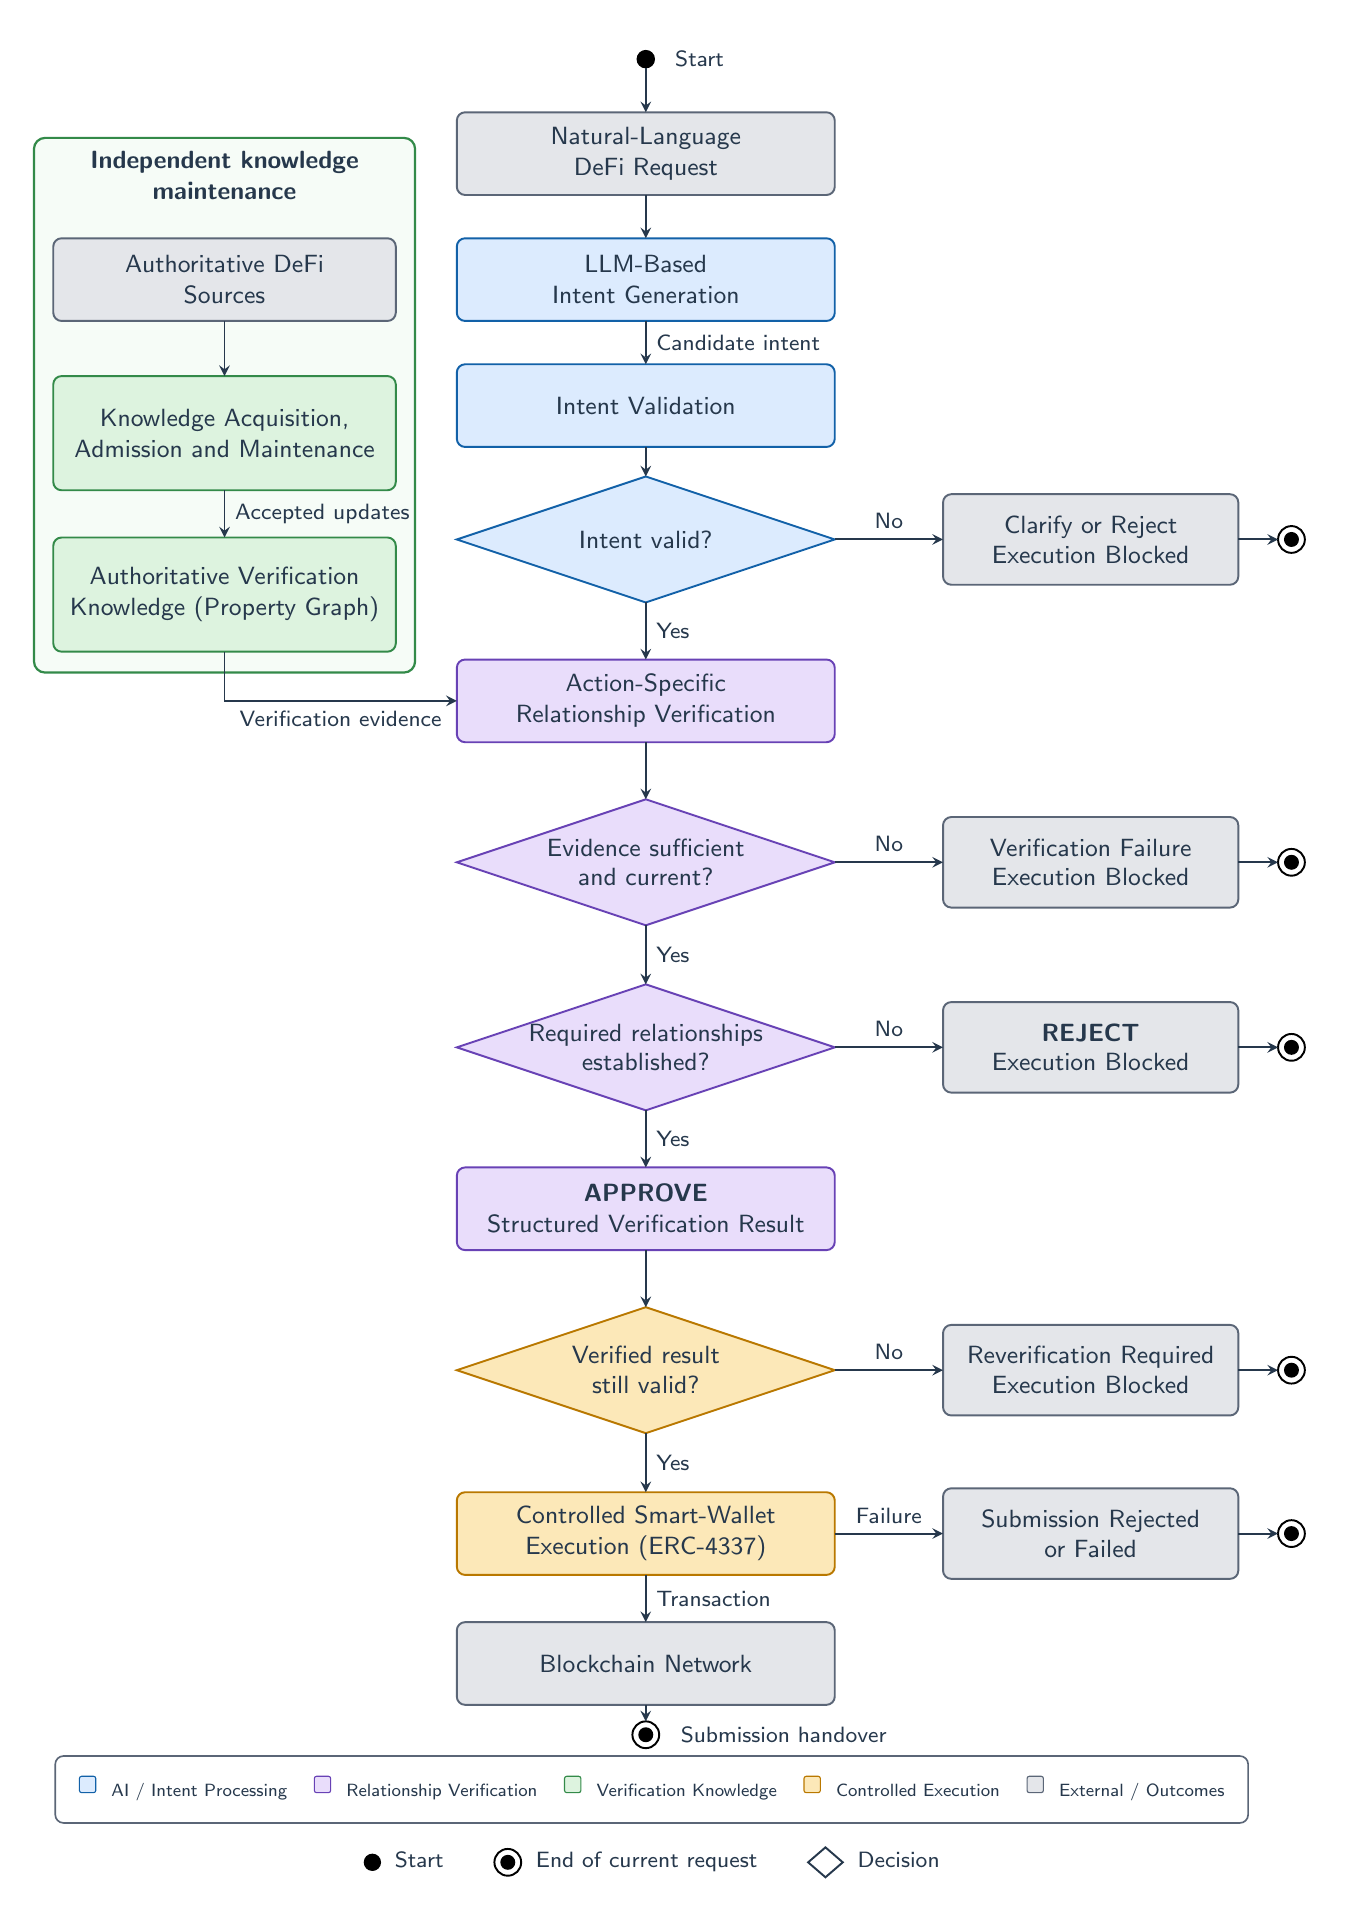
\begin{tikzpicture}[x=1cm,y=1cm,>=stealth]
\path[use as bounding box] (0,-0.20) rectangle (16.55,23.45);

% Subsystem colours, consistent with the component diagram.
\definecolor{archline}{HTML}{26384C}
\definecolor{aiborder}{HTML}{1261A8}
\definecolor{aifill}{HTML}{DCEBFE}
\definecolor{verborder}{HTML}{6842B5}
\definecolor{verfill}{HTML}{E9DDFB}
\definecolor{knowborder}{HTML}{338A49}
\definecolor{knowfill}{HTML}{DDF3DF}
\definecolor{execborder}{HTML}{B97800}
\definecolor{execfill}{HTML}{FCE8B8}
\definecolor{extborder}{HTML}{5B6677}
\definecolor{extfill}{HTML}{E4E6EA}

\tikzset{
  flowbox/.style={rectangle,rounded corners=3pt,line width=0.7pt,
    align=center,text=archline,font=\sffamily\fontsize{9.3}{11.2}\selectfont,
    text width=4.30cm,minimum width=4.80cm,minimum height=1.05cm,
    inner xsep=3pt,inner ysep=3pt,outer sep=0pt},
  ai/.style={flowbox,draw=aiborder,fill=aifill},
  verification/.style={flowbox,draw=verborder,fill=verfill},
  execution/.style={flowbox,draw=execborder,fill=execfill},
  external/.style={flowbox,draw=extborder,fill=extfill},
  knowledge/.style={flowbox,draw=knowborder,fill=knowfill,
    text width=3.95cm,minimum width=4.35cm,minimum height=1.45cm},
  outcome/.style={external,text width=3.35cm,minimum width=3.75cm,
    minimum height=1.15cm,font=\sffamily\fontsize{9}{10.8}\selectfont},
  flowarrow/.style={->,draw=archline,line width=0.70pt},
  arrowlabel/.style={font=\sffamily\fontsize{7.8}{9.2}\selectfont,
    text=archline,fill=none,inner sep=0.8pt,outer sep=0pt},
  annotation/.style={align=center,text=archline,
    font=\sffamily\fontsize{8.4}{10}\selectfont}
}

% Diamond dimensions and predictable connection points.
% Arguments: name, y, border colour, fill colour, text.
\def\FlowDecision#1#2#3#4#5{%
  \draw[draw=#3,fill=#4,line width=0.7pt]
    (7.85,{#2+0.80}) -- (10.25,#2) --
    (7.85,{#2-0.80}) -- (5.45,#2) -- cycle;
  \node[align=center,text=archline,text width=3.40cm,
    font=\sffamily\fontsize{9.0}{10.8}\selectfont,inner sep=0pt]
    at (7.85,#2) {#5};
  \coordinate (#1-north) at (7.85,{#2+0.80});
  \coordinate (#1-south) at (7.85,{#2-0.80});
  \coordinate (#1-east) at (10.25,#2);
}

% =========================================================
% Main request-processing path
% =========================================================
% UML-style initial node for one request-processing attempt.
\node[circle,draw=black,fill=black,minimum size=0.22cm,
  inner sep=0pt,outer sep=0pt] (requeststart) at (7.85,23.05) {};
\node[annotation,anchor=west] at (8.10,23.05) {Start};

\node[external] (request) at (7.85,21.85)
  {Natural-Language\\DeFi Request};
\node[ai] (generation) at (7.85,20.25)
  {LLM-Based\\Intent Generation};
\node[ai] (validation) at (7.85,18.65)
  {Intent Validation};
\FlowDecision{intent}{16.95}{aiborder}{aifill}
  {Intent valid?}

\draw[flowarrow] (requeststart.south) -- (request.north);
\draw[flowarrow] (request.south) -- (generation.north);
\draw[flowarrow] (generation.south) --
  node[arrowlabel,pos=0.5,right=3pt] {Candidate intent}
  (validation.north);
\draw[flowarrow] (validation.south) -- (intent-north);

\node[outcome] (intentfailure) at (13.50,16.95)
  {Clarify or Reject\\Execution Blocked};
\draw[flowarrow] (intent-east) --
  node[arrowlabel,pos=0.5,above=3pt] {No} (intentfailure.west);

\node[verification] (verify) at (7.85,14.90)
  {Action-Specific\\Relationship Verification};
\draw[flowarrow] (intent-south) --
  node[arrowlabel,pos=0.5,right=3pt] {Yes} (verify.north);

\FlowDecision{evidence}{12.85}{verborder}{verfill}
  {Evidence sufficient\\and current?}
\draw[flowarrow] (verify.south) -- (evidence-north);
\node[outcome] (insufficient) at (13.50,12.85)
  {Verification Failure\\Execution Blocked};
\draw[flowarrow] (evidence-east) --
  node[arrowlabel,pos=0.5,above=3pt] {No} (insufficient.west);

\FlowDecision{relationships}{10.50}{verborder}{verfill}
  {Required relationships\\established?}
\draw[flowarrow] (evidence-south) --
  node[arrowlabel,pos=0.5,right=3pt] {Yes} (relationships-north);
\node[outcome] (rejection) at (13.50,10.50)
  {\textbf{REJECT}\\Execution Blocked};
\draw[flowarrow] (relationships-east) --
  node[arrowlabel,pos=0.5,above=3pt] {No} (rejection.west);

\node[verification] (approved) at (7.85,8.45)
  {\textbf{APPROVE}\\Structured Verification Result};
\draw[flowarrow] (relationships-south) --
  node[arrowlabel,pos=0.5,right=3pt] {Yes} (approved.north);

% Includes the pre-execution check of the approved result.
\FlowDecision{valid}{6.40}{execborder}{execfill}
  {Verified result\\still valid?}
\draw[flowarrow] (approved.south) -- (valid-north);
\node[outcome] (reverify) at (13.50,6.40)
  {Reverification Required\\Execution Blocked};
\draw[flowarrow] (valid-east) --
  node[arrowlabel,pos=0.5,above=3pt] {No} (reverify.west);

\node[execution] (execution) at (7.85,4.325)
  {Controlled Smart-Wallet\\Execution (ERC-4337)};
\draw[flowarrow] (valid-south) --
  node[arrowlabel,pos=0.5,right=3pt] {Yes} (execution.north);
\node[outcome] (submissionfailure) at (13.50,4.325)
  {Submission Rejected\\or Failed};
\draw[flowarrow] (execution.east) --
  node[arrowlabel,pos=0.5,above=3pt] {Failure} (submissionfailure.west);

\node[external] (chain) at (7.85,2.675)
  {Blockchain Network};
\draw[flowarrow] (execution.south) --
  node[arrowlabel,pos=0.5,right=3pt] {Transaction} (chain.north);

% UML-style activity-final nodes end the current request attempt.
% They do not stop the independently maintained knowledge subsystem.
\def\FlowRequestEnd#1#2#3{%
  \node[circle,draw=black,fill=white,line width=0.7pt,
    minimum size=0.34cm,inner sep=0pt,outer sep=0pt]
    (#1) at (#2,#3) {};
  \fill[black] (#1.center) circle[radius=0.095cm];
}

\FlowRequestEnd{intentend}{16.05}{16.95}
\draw[flowarrow] (intentfailure.east) -- (intentend.west);

\FlowRequestEnd{evidenceend}{16.05}{12.85}
\draw[flowarrow] (insufficient.east) -- (evidenceend.west);

\FlowRequestEnd{rejectionend}{16.05}{10.50}
\draw[flowarrow] (rejection.east) -- (rejectionend.west);

\FlowRequestEnd{reverifyend}{16.05}{6.40}
\draw[flowarrow] (reverify.east) -- (reverifyend.west);

\FlowRequestEnd{submissionend}{16.05}{4.325}
\draw[flowarrow] (submissionfailure.east) -- (submissionend.west);

% This endpoint denotes handover for submission, not confirmed execution.
\FlowRequestEnd{handoverend}{7.85}{1.77}
\draw[flowarrow] (chain.south) -- (handoverend.north);
\node[annotation,anchor=west] at (8.17,1.77) {Submission handover};

% % =========================================================
% % Independent knowledge branch
% % =========================================================
% \node[external,text width=3.95cm,minimum width=4.35cm]
%   (sources) at (2.50,20.25) {Authoritative DeFi\\Sources};
% \node[knowledge] (acquisition) at (2.50,18.30)
%   {Knowledge Acquisition,\\Admission and\\Maintenance};
% \node[knowledge] (graph) at (2.50,16.25)
%   {Authoritative Verification\\Knowledge\\(Property Graph)};
% \draw[flowarrow] (sources.south) -- (acquisition.north);
% \draw[flowarrow] (acquisition.south) --
%   node[arrowlabel,pos=0.5,left=3pt] {Accepted updates} (graph.north);
% \draw[flowarrow] (graph.east) -- (5.075,16.25) --
%   (5.075,14.90) -- (verify.west);
% \node[annotation,text width=4.20cm] at (2.50,14.45)
%   {Maintained independently};

% =========================================================
% Independent knowledge maintenance
% =========================================================

% Separate panel: this process runs independently of user requests.
\draw[
  draw=knowborder,
  fill=knowfill!25!white,
  rounded corners=4pt,
  line width=0.8pt
] (0.08,15.26) rectangle (4.92,22.05);

\node[
  align=center,
  text=archline,
  font=\sffamily\bfseries\fontsize{9.3}{11.2}\selectfont,
  inner sep=0pt
] at (2.50,21.58) {Independent knowledge \\ maintenance};

% Existing knowledge stages, in their original colours.
\node[external,text width=3.95cm,minimum width=4.35cm]
  (sources) at (2.50,20.25)
  {Authoritative DeFi\\Sources};

\node[knowledge]
  (acquisition) at (2.50,18.30)
  {Knowledge Acquisition,\\Admission and Maintenance};

\node[knowledge]
  (graph) at (2.50,16.25)
  {Authoritative Verification\\Knowledge (Property Graph)};

\draw[flowarrow]
  (sources.south) -- (acquisition.north);

\draw[flowarrow]
  (acquisition.south) --
  node[arrowlabel,midway,right=3pt] {Accepted updates}
  (graph.north);

% The verifier uses evidence from the maintained graph.
% Route below the panel so the label stays clear of its border.
\draw[flowarrow]
  (graph.south) -- (2.50,14.90) --
  node[arrowlabel,midway,below=3pt] {Verification evidence}
  (verify.west);

% =========================================================
% One-row legend: aligned swatches and labels
% =========================================================
\begingroup

\def\LegendSwatch#1#2{%
  \tikz[baseline=-0.5ex]{%
    \draw[
      draw=#1,
      fill=#2,
      rounded corners=1pt,
      line width=0.5pt
    ] (0,0) rectangle (0.26,0.26);
  }%
  \hspace{4pt}%
}

\draw[draw=extborder,rounded corners=3pt,line width=0.6pt]
  (0.35,0.65) rectangle (15.50,1.50);

\node[
  font=\sffamily\fontsize{8.5}{10}\selectfont,
  text=archline,
  inner sep=0pt,
  outer sep=0pt
] at (7.925,1.075) {%
  \resizebox{14.55cm}{!}{%
    \begin{tabular}{
      @{}l@{\hspace{12pt}}
      l@{\hspace{12pt}}
      l@{\hspace{12pt}}
      l@{\hspace{12pt}}
      l@{}
    }
      \LegendSwatch{aiborder}{aifill} AI / Intent Processing
      &
      \LegendSwatch{verborder}{verfill} Relationship Verification
      &
      \LegendSwatch{knowborder}{knowfill} Verification Knowledge
      &
      \LegendSwatch{execborder}{execfill} Controlled Execution
      &
      \LegendSwatch{extborder}{extfill} External / Outcomes
    \end{tabular}%
  }%
};

\endgroup

% Compact, centred UML-style notation key
\node[
  annotation,
  inner sep=0pt,
  outer sep=0pt
] at (7.925,0.15) {%
  \begin{tabular}{
    @{}c@{\hspace{5pt}}l
    @{\hspace{18pt}}
    c@{\hspace{5pt}}l
    @{\hspace{18pt}}
    c@{\hspace{5pt}}l@{}
  }
    % Start
    \tikz[baseline=-0.5ex]{
      \fill[black] (0,0) circle[radius=0.11cm];
    }
    & Start
    &
    % End
    \tikz[baseline=-0.5ex]{
      \draw[draw=black,fill=white,line width=0.7pt]
        (0,0) circle[radius=0.17cm];
      \fill[black] (0,0) circle[radius=0.095cm];
    }
    & End of current request
    &
    % Decision
    \tikz[baseline=-0.5ex]{
      \draw[draw=archline,fill=white,line width=0.7pt]
        (0,0.19) -- (0.22,0) -- (0,-0.19) --
        (-0.22,0) -- cycle;
    }
    & Decision
  \end{tabular}%
};

\end{tikzpicture}
\endgroup%
    }
    \caption{Overall request-processing flow and supporting knowledge
    maintenance.}
    \label{fig:overall_system_flow}
\end{figure}
The language model converts the natural-language
request into a candidate intent, which must pass validation before
relationship verification begins. Validation checks whether the intent is
complete, valid, supported, and unambiguous. Requests that do not satisfy
these conditions require clarification or are rejected, and execution is
blocked.


The supporting knowledge branch shows how the authoritative property graph
is established and maintained independently of individual requests.
Information from authoritative DeFi sources, including official protocol
documentation, deployment records, and blockchain data, is acquired and
assessed for authority, consistency, and freshness before accepted entities
and relationships are added or updated. The maintained graph provides the
reference relationships and evidence used during verification.

Relationship verification evaluates the action-specific relationships
required by the validated intent. Approval requires sufficient and current
evidence establishing all mandatory relationships. If the evidence is
incomplete, stale, or unavailable, verification fails without approval.
Missing or inconsistent relationships support rejection only when the
applicable knowledge is sufficiently complete and current. An
\texttt{APPROVE} decision therefore indicates consistency with the
represented authoritative relationships within the supported scope; it does
not guarantee successful blockchain execution.

Controlled smart-wallet execution consumes the approved structured
verification result. Before submission, it checks that the
protected parameters remain unchanged, the approval has not expired, and
the referenced verification evidence remains applicable. If these conditions
are not satisfied, execution is blocked and renewed verification is required.
Even when the result remains valid, wallet authorization or execution-layer
validation may prevent successful submission. Such submission failures remain
distinct from the graph-verification decision. The blockchain endpoint in the
figure denotes submission rather than confirmation that the requested
operation has completed successfully.


It determines whether the action-specific execution relationships required
by the request can be established consistently and produces an approval,
rejection, or verification failure together with the relevant evidence
or failure reason.

Figure~\ref{fig:system_architecture} shows how the five conceptual elements
are organized into four subsystems. The arrows show the information exchanged
between them. Relationship Verification receives two inputs: a validated
intent from AI / Intent Processing, which interprets and validates the user's
request, and verification evidence from Verification Knowledge, which maintains
the authoritative property graph using records from DeFi sources. The verifier
uses this evidence to check the relationships required by the requested action.
Only an approved verification result is passed to Controlled Execution, which
checks that the approval remains valid before submitting the operation to the
blockchain network.

\begin{figure}[H]
    \centering
    \resizebox{0.98\textwidth}{!}{%
        

% All information flows point from sender to receiver; see notation key.
\begingroup
\definecolor{archline}{HTML}{2F425A}
\definecolor{archtext}{HTML}{1E293B}
\definecolor{aiborder}{HTML}{1261A8}
\definecolor{aifill}{HTML}{DCEBFE}
\definecolor{knowborder}{HTML}{26864A}
\definecolor{knowfill}{HTML}{E1F4E5}
\definecolor{verborder}{HTML}{3F2C8C}
\definecolor{verfill}{HTML}{EAE6FA}
\definecolor{execborder}{HTML}{B86F00}
\definecolor{execfill}{HTML}{FEEDCD}
\definecolor{extborder}{HTML}{44556B}
\definecolor{extfill}{HTML}{DCDDE2}

\usetikzlibrary{arrows}
\begin{tikzpicture}[x=1cm,y=1cm,
 every node/.style={text=archtext,font=\sffamily\small,align=center},
 infoflow/.style={->,>=angle 60,draw=archline,dash pattern=on 4pt off 2.5pt,line width=.78pt},
 assoc/.style={draw=archline,line width=.78pt},
 labeltext/.style={font=\sffamily\footnotesize,inner sep=2pt},
 ext/.style={draw=extborder,fill=extfill,minimum width=3.55cm,
   minimum height=.75cm,inner sep=2pt,outer sep=0pt}]
% UML component glyph: a classifier rectangle with two protruding tabs.
\def\ArchGlyph#1#2#3{%
  \begin{scope}[shift={(#1,#2)},draw=archline,line width=.6pt]
    \draw[fill=#3] (-.18,-.14) rectangle (.18,.14);
    \draw[fill=#3] (-.25,.035) rectangle (-.10,.095);
    \draw[fill=#3] (-.25,-.095) rectangle (-.10,-.035);
  \end{scope}}
% The four equal component symbols have a header and a responsibility list.
% Parameters: name, x, y, outline, fill, title, responsibilities.
\def\ArchComponent#1#2#3#4#5#6#7{%
  \node[rectangle,draw=#4,fill=#5,line width=.85pt,
     minimum width=5.10cm,minimum height=2.55cm,inner sep=0pt,
     outer sep=0pt] (#1) at (#2,#3) {};
  \begin{scope}[shift={(#1.center)}]
    \ArchGlyph{2.12}{.96}{#5}
    \node[font=\sffamily\bfseries\small,inner sep=0pt] at (0,.55) {#6};
    \draw[draw=#4,line width=.55pt] (-2.55,.08) -- (2.55,.08);
    \node[inner sep=0pt,font=\sffamily\fontsize{8.1}{10.8}\selectfont] at (0,-.57) {#7};
  \end{scope}}
\draw[draw=extborder,line width=.85pt] (0,1.7) rectangle (15.1,10.65);
\node[anchor=center,fill=white,inner xsep=5pt,font=\sffamily\bfseries\small]
 at (7.55,10.65) {AI-assisted DeFi verification system};

\ArchComponent{ai}{3.1}{8.57}{aiborder}{aifill}{AI / Intent Processing}
  {LLM-based intent generation\\Intent validation}
\ArchComponent{knowledge}{12.0}{8.57}{knowborder}{knowfill}{Verification Knowledge}
  {Acquire and maintain knowledge\\Authoritative property graph}
\ArchComponent{verifier}{3.1}{3.70}{verborder}{verfill}{Relationship Verification}
  {Action-specific relationship checks\\Verification decision and evidence}
\ArchComponent{exec}{12.0}{3.70}{execborder}{execfill}{Controlled Execution}
  {Verified-result validity check\\ERC-4337 smart-wallet execution}

% External entities.
\node[ext] (user) at (3.1,11.83) {User};
\node[ext] (sources) at (12,11.83) {Authoritative DeFi sources};
\node[ext] (chain) at (12,.61) {Blockchain network};

% Labels identify the information conveyed, rather than the calling component.
\draw[infoflow] (user.south) -- (ai.north);
\node[labeltext,anchor=west] at (3.18,11.04) {DeFi request};
\draw[infoflow] (sources.south) -- (knowledge.north);
\node[labeltext,anchor=east] at (11.91,11.04) {Protocol and deployment records};

% The verifier has two independent inputs, with distinct arrow endpoints.
\draw[infoflow] (ai.south) -- (verifier.north);
\node[labeltext,anchor=east] at (3.00,6.13) {Validated intent};
\draw[infoflow] (knowledge.south) -- (12.0,6.27) -- (4.95,6.27)
  -- (4.95,4.975);
\node[labeltext,anchor=south] at (8.48,6.34) {Verification evidence};
\draw[infoflow] (verifier.east) -- (exec.west);
\node[labeltext,anchor=south] at (7.55,3.80) {Approved\\verification result};
\draw[infoflow] (exec.south) -- (chain.north);
\node[labeltext,anchor=east] at (11.91,1.35) {Operation for submission};

% One-row colour legend, with a separate notation key underneath.
\draw[draw=extborder!65,rounded corners=2pt,line width=.55pt]
  (0,-1.88) rectangle (15.10,-.13);
\def\ArchSwatch#1#2{%
  \tikz[baseline=-.48ex]{\draw[draw=#1,fill=#2,line width=.55pt]
       (0,0) rectangle (.22,.22);}\hspace{3pt}}
\node[inner sep=0pt,font=\sffamily\fontsize{7.4}{9.2}\selectfont]
 at (7.55,-.54) {\makebox[14.50cm][s]{%
  \ArchSwatch{aiborder}{aifill}AI / Intent Processing\hfill
  \ArchSwatch{verborder}{verfill}Relationship Verification\hfill
  \ArchSwatch{knowborder}{knowfill}Verification Knowledge\hfill
  \ArchSwatch{execborder}{execfill}Controlled Execution\hfill
  \ArchSwatch{extborder}{extfill}External Environment}};
\draw[draw=extborder!35,line width=.4pt] (.27,-.96) -- (14.83,-.96);
\ArchGlyph{3.0}{-1.42}{white}
\node[labeltext,anchor=west] at (3.29,-1.42) {System component};
\draw[infoflow] (7.41,-1.42) -- (8.25,-1.42);
\node[labeltext,anchor=west] at (8.42,-1.42)
  {Information flow (sender to receiver)};
\end{tikzpicture}
\endgroup%
    }
   \caption{component diagram of the AI-assisted DeFi verification system.}
    \label{fig:system_architecture}
\end{figure}



% =========================================================
% 3.2 LLM-Based Intent Generation
% =========================================================

\section{LLM-Based Intent Generation}
\label{sec:intent_generation}

The first processing element converts the user's natural-language DeFi request
into a machine-readable representation. For example, a user may submit the
following request:

\begin{quote}
\textit{``Swap 50 USDT for WETH using Uniswap V3.''}
\end{quote}

In this example, the requested action is a swap, the protocol is Uniswap V3,
the input asset is USDT, the output asset is WETH, and the amount is 50 USDT.
Although these parameters are expressed in natural language, they must be
organized into a structured representation before they can be evaluated by
the relationship-verification component. The language model therefore
interprets the request, extracts this user-level information, and organizes
it according to a predefined structured-intent model.

Structured generation provides a predictable interface between probabilistic
language interpretation and subsequent deterministic processing. Constraining
language-model output to an expected structure can reduce variability in
generated outputs and improve their suitability for downstream processing
\cite{geng2023grammar}. Nevertheless, the generated output is treated only as
a \textit{candidate structured intent}; it is not trusted directly for
blockchain execution.

The information extracted in the example illustrates the general purpose of
the structured-intent model. At the conceptual level, a candidate intent may
contain the fields shown in Table~\ref{tab:structured_intent_fields}.


\begin{table}[H]
\centering
\small
\caption{Conceptual fields of the structured DeFi intent, with values
extracted from ``Swap 50 USDT for WETH using Uniswap V3.''}
\label{tab:structured_intent_fields}

\begin{tabular}{@{}p{0.20\textwidth} p{0.55\textwidth} p{0.16\textwidth}@{}}
\hline
\textbf{Field} & \textbf{Purpose} & \textbf{Value} \\
\hline

Action &
Requested DeFi operation, such as swap, supply, withdraw, or borrow. &
Swap \\

Protocol &
Requested DeFi protocol when explicitly specified or required by the
supported operation. &
Uniswap V3 \\

Network &
Blockchain network on which the operation is intended to take place. &
Not specified \\

Input / Asset &
Asset provided, supplied, withdrawn, or borrowed depending on the action. &
USDT \\

Output Asset &
Asset expected from an exchange operation, where applicable. &
WETH \\

Amount &
Quantity associated with the requested operation. &
50 USDT \\

Recipient / Spender &
Destination or authorization-related entity where required. &
Not specified \\

Action-Specific Data &
Additional user-level parameters required by a particular supported action. &
Not specified \\

\hline
\end{tabular}
\end{table}

The required fields depend on the requested action. A swap requires an input
asset, output asset, and amount, whereas a supply operation requires an asset
and amount but no output asset. The example request does not explicitly
specify a network. The network context may be specified by the user or
provided by the execution environment. In either case, it must be established
before relationship verification because protocol deployments and their
associated execution resources are network-specific.

The candidate intent describes \textit{what the user requests}, but does not
require the language model to select the final contract address, callable
function, liquidity pool, or transaction payload. These execution-specific
elements are resolved later using authoritative verification knowledge.
Whether the candidate intent is sufficiently complete, supported, and
unambiguous is determined by the intent-validation component described in
the following section.

% =========================================================
% 3.3 Intent Validation
% =========================================================

\section{Intent Validation}
\label{sec:intent_validation}

The candidate intent generated by the language model must be validated before
it is used for relationship verification. The purpose of this stage is to
determine whether the structured representation is sufficiently complete,
well-formed, supported, and unambiguous for deterministic processing. General schema-validation mechanisms commonly support checks such as required
properties, data types, permitted values, and numerical bounds
\cite{jsonschema2020}. In the proposed concept, these structural checks are
combined with action-specific and contextual DeFi checks.

Four categories of validation are considered:

\begin{enumerate}

    \item \textbf{Structural validation} checks whether the candidate follows
    the expected representation and contains the required fields in an
    appropriate form.

    \item \textbf{Action-specific validation} determines whether the fields
    required for the selected operation are present. For example, a swap
    requires both input and output assets, whereas a supply request requires
    an asset and amount.

    \item \textbf{Value validation} checks basic constraints on individual
    values. An amount, for example, must represent a permitted positive
    quantity.

    \item \textbf{Context and ambiguity validation} checks whether the
    requested action and network are within the supported scope and whether
    critical identifiers can be resolved unambiguously. An ambiguous asset
    identifier must not be resolved by guessing.

\end{enumerate}

If all required conditions are satisfied, the candidate becomes a
\textit{validated structured intent} and may proceed to relationship
verification. Missing, malformed, unsupported, or unresolved information
prevents further processing. Depending on the interaction model, the system may
request clarification from the user or reject the request. For the example swap request, validation checks whether the input asset, output
asset, and amount are present, whether the amount is permitted, whether the
action and network are supported, and whether the asset identifiers can be
interpreted unambiguously. It does not determine the router contract, callable
function, or liquidity pool.

Deterministic validation has a defined limitation. A structurally complete and
internally valid intent does not prove that the language model has perfectly
interpreted the user's meaning. The validation stage can identify missing,
invalid, unsupported, or ambiguous information, but it cannot generally prove
semantic equivalence between the original natural-language request and the
generated representation. The subsequent verification therefore assumes that
the validated intent represents the requested operation and focuses on whether
an authoritative execution structure can be established for it.


% =========================================================
% 3.4 Authoritative Verification Knowledge and Graph Model
% =========================================================

\section{Authoritative Verification Knowledge and Graph Model}
\label{sec:verification_knowledge}

Before a validated intent can be verified, the system requires an
authoritative representation of the execution relationships supported by
the relevant DeFi protocols. This verification knowledge is acquired,
checked, and maintained independently of the language model and individual
user requests. It represents accepted information about protocol deployments,
supported actions, contracts, callable functions, assets, liquidity pools,
lending reserves, and their relationships within the supported scope.

A graph-based representation is used because verification depends not only
on the validity of individual entities but also on their relationships.
For example, a legitimate contract or asset is insufficient if it does
not belong to the protocol deployment and action required by the current
request. The following subsections explain how this knowledge is established,
represented, and maintained for use by the relationship-verification component
described in Section~\ref{sec:relationship_verification}.

\subsection{Knowledge Acquisition and Admission}

The graph is constructed from authoritative protocol and blockchain information
rather than from execution information generated by the language model.
Relevant sources may include official deployment information, contract or
address registries, protocol-defined interfaces and documentation, and directly
verifiable on-chain protocol state. These sources provide the deployment, contract, function, asset, and
protocol-resource information required to construct the verification graph.
Table~\ref{tab:verification_sources} summarizes the main information categories
and their role in the graph. Examples include the network-specific deployment records published for Uniswap V3 and the contract addresses maintained in the Aave Address Book \cite{UniswapV3Deployments,AaveAddressBook}.

\begin{table}[H]
\centering
\caption{Conceptual sources of authoritative verification knowledge.}
\label{tab:verification_sources}
\small
\begin{tabular}{p{0.30\textwidth} p{0.29\textwidth} p{0.33\textwidth}}
\hline
\textbf{Information} &
\textbf{Source Category} &
\textbf{Purpose in the Graph} \\
\hline

Protocol deployment &
Official deployment information or registry &
Identifies network, version, and deployment context. \\

Contract information &
Official contract or address information &
Associates authoritative contracts with a deployment. \\

Callable functions &
Protocol-defined interfaces or documentation &
Associates functions with supported protocol actions. \\

Liquidity pools &
Verifiable protocol or on-chain state &
Associates pools with deployments, assets, and pool configuration. \\

Lending reserves &
Verifiable protocol or on-chain state &
Associates reserves with deployments and underlying assets. \\

Asset information &
Accepted protocol- or network-specific information &
Identifies assets in the correct blockchain context. \\

\hline
\end{tabular}
\end{table}

An important distinction is made between \textit{discovered information} and
\textit{accepted verification information}. Discovering an entity does not by
itself make that entity suitable for approving an execution. Before information
is admitted to the verification knowledge, its applicable context must be
established. Depending on the information type, this includes the originating
source, blockchain network, protocol and version, associated deployment,
synchronization time, and validity state.

Information whose source or applicable context cannot be established is not
used as positive verification evidence. The acquisition process can therefore
be summarized as:
\begin{figure}[H]
\centering
\resizebox{\linewidth}{!}{%

\begin{tikzpicture}[x=1cm,y=1cm,>=stealth]

% Colours
\definecolor{stepfill}{HTML}{F8FAFC}
\definecolor{stepborder}{HTML}{475569}
\definecolor{arrowcol}{HTML}{64748B}
\definecolor{steptext}{HTML}{1E293B}

% Authoritative Source
\draw[rounded corners=0.08cm, draw=stepborder,
      fill=stepfill, line width=0.6pt]
  (0,0) rectangle (3.2,1.1);
\node[align=center, text=steptext, font=\small]
  at (1.6,0.55)
  {\textit{Authoritative}\\\textit{Source}};

% Acquire
\draw[rounded corners=0.08cm, draw=stepborder,
      fill=stepfill, line width=0.6pt]
  (4.0,0) rectangle (6.2,1.1);
\node[align=center, text=steptext, font=\small]
  at (5.1,0.55)
  {\textit{Acquire}};

% Contextualize and Validate
\draw[rounded corners=0.08cm, draw=stepborder,
      fill=stepfill, line width=0.6pt]
  (7.55,0) rectangle (10.35,1.1);
\node[align=center, text=steptext, font=\small]
  at (8.95,0.55)
  {\textit{Contextualize}\\\textit{and Validate}};

% Admit as Verification Knowledge
\draw[rounded corners=0.08cm, draw=stepborder,
      fill=stepfill, line width=0.6pt]
  (11.7,0) rectangle (15.4,1.1);
\node[align=center, text=steptext, font=\small]
  at (13.55,0.55)
  {\textit{Admit as}\\\textit{Verification Knowledge}};

% Arrows connected to box edges
\draw[->, line width=0.7pt, draw=arrowcol]
  (3.2,0.55) -- (4.0,0.55);

\draw[->, line width=0.7pt, draw=arrowcol]
  (6.2,0.55) -- (7.55,0.55);

\draw[->, line width=0.7pt, draw=arrowcol]
  (10.35,0.55) -- (11.7,0.55);

\end{tikzpicture}%
}
\caption{Conceptual stages in establishing authoritative verification knowledge.}
\label{fig:knowledge_admission_flow}
\end{figure}

Knowledge acquisition continues after the graph is first populated and
takes place independently of individual user requests. During each
synchronization, the system compares information from authoritative sources
with the accepted records for the same network and protocol deployment.
New or changed information must meet the same admission criteria as the
original records. If a source confirms that a previously accepted
relationship is no longer valid, that relationship can no longer support
approval. If a source cannot be reached, the failed check does not renew
the freshness of the existing record.


The exact acquisition scripts, API calls, blockchain queries, and storage
operations are implementation concerns and are described in Chapter~\ref{chap:implementation}.

\subsection{Graph Model and Maintenance}
A property graph represents entities as nodes and their relationships as
edges; both can carry properties \cite{angles2018propertygraph}. In the
proposed model, nodes represent entities such as protocol deployments,
actions, contracts, and assets. The edges identify which deployment
supports an action, which contract exposes a function, and which assets
belong to a pool. Table~\ref{tab:graph_entities} summarizes the principal
entities.

\begin{table}[H]
\centering
\caption{Principal entities in the authoritative verification knowledge.}
\label{tab:graph_entities}
\small
\begin{tabular}{p{0.29\textwidth} p{0.66\textwidth}}
\hline
\textbf{Entity} & \textbf{Purpose} \\
\hline

Blockchain Network &
Defines the network context of a protocol deployment. \\

Protocol Deployment &
Represents a protocol deployment or version on a particular network. \\

Action &
Represents a supported DeFi operation such as swap, supply, withdraw, or
borrow. \\

Authoritative Contract &
Represents a contract accepted for the applicable protocol deployment. \\

Callable Function &
Represents a contract function associated with a supported action. \\

Asset &
Represents an asset in its applicable network context. \\

Liquidity Pool &
Represents an exchange resource and its participating assets and
configuration. \\

Reserve &
Represents a lending resource associated with an underlying asset. \\

Protocol-Specific Resource &
Represents additional resources required by a particular protocol or action. \\

\hline
\end{tabular}
\end{table}

Conceptually, the graph represents relationships such as a network hosting a
protocol deployment, a deployment supporting an action, a deployment using an
authoritative contract, a contract exposing a callable function, and a function
implementing an action. Additional branches associate deployments with
liquidity pools, reserves, assets, and other protocol-specific resources.

Knowledge completeness is assessed within a defined verification scope,
such as a particular network, protocol deployment, action, and resource
category. Freshness is assessed using the applicable update policy and
the recorded synchronization and validity information. A synchronization
timestamp alone does not establish that all required knowledge has been
acquired. If sufficient coverage or current applicability cannot be
established, missing relationships are treated as insufficient evidence.



\begin{figure}[H]
    \centering
    \resizebox{0.95\textwidth}{!}{%
        \begingroup
\hyphenpenalty=10000
\exhyphenpenalty=10000
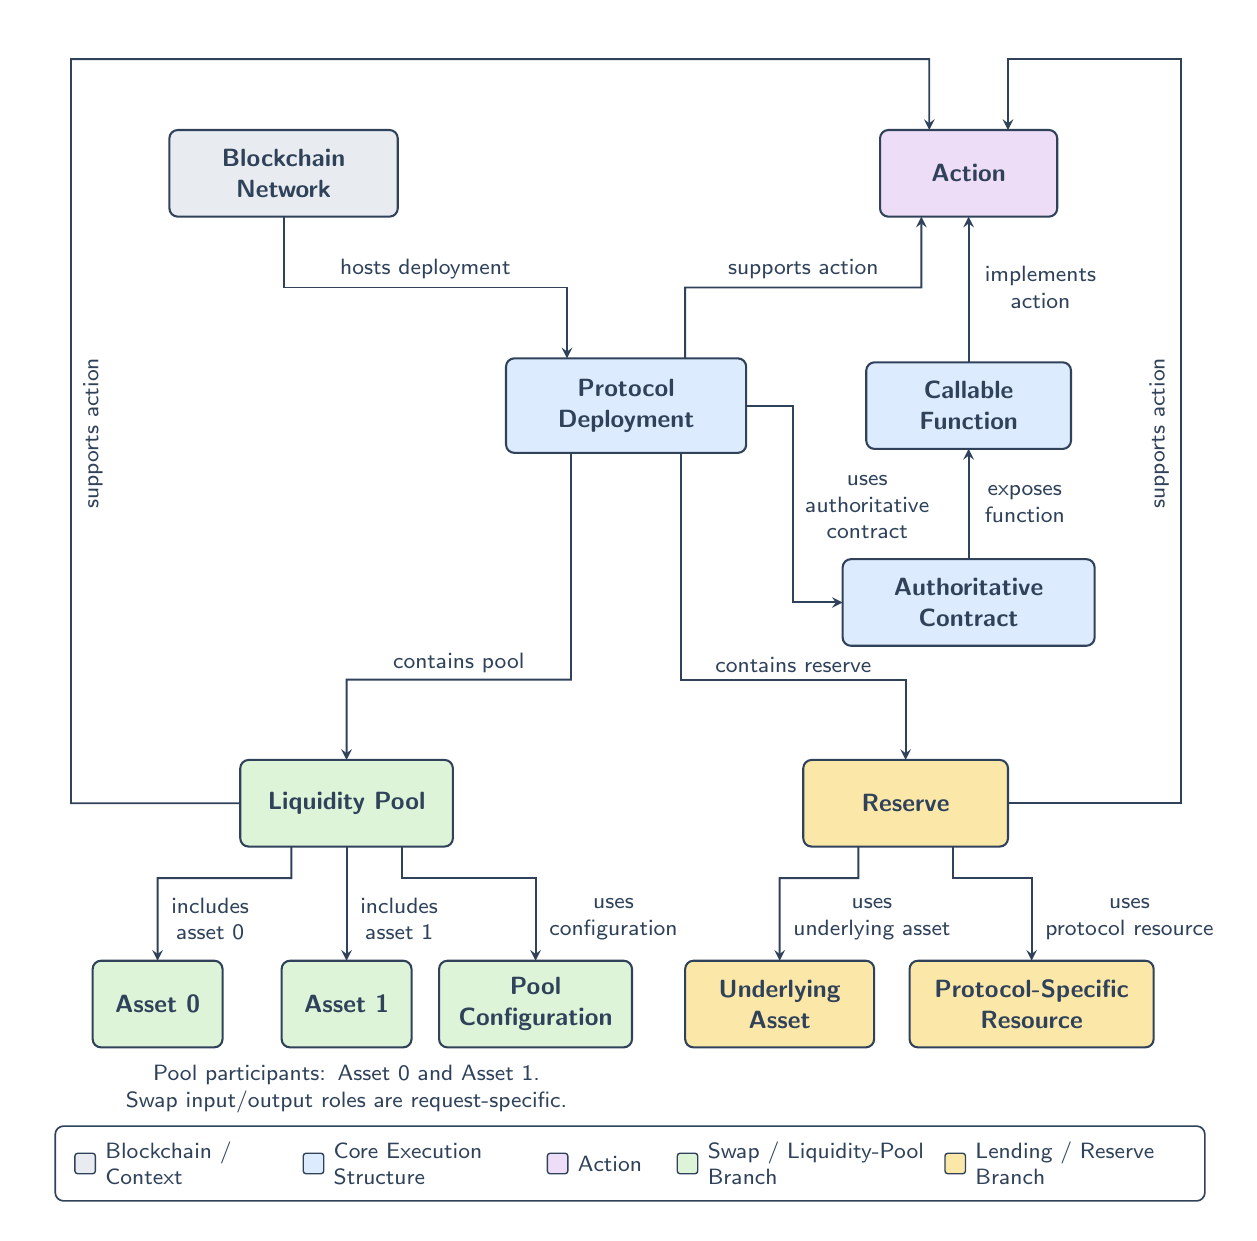
\begin{tikzpicture}[x=1cm,y=1cm,>=stealth]
\path[use as bounding box] (0,0) rectangle (15.25,15.05);

\definecolor{graphline}{HTML}{2F425A}
\definecolor{contextfill}{HTML}{E8ECF0}
\definecolor{corefill}{HTML}{DCEBFE}
\definecolor{actionfill}{HTML}{EEDDF6}
\definecolor{swapfill}{HTML}{DDF4D9}
\definecolor{lendfill}{HTML}{FBE8A9}

\tikzset{
  entity/.style={rectangle,rounded corners=3pt,draw=graphline,
    line width=0.75pt,align=center,text=graphline,
    inner xsep=4pt,inner ysep=4pt,outer sep=0pt,
    font=\sffamily\bfseries\fontsize{9.4}{11.2}\selectfont},
  relation/.style={->,draw=graphline,line width=0.70pt},
  relationlabel/.style={text=graphline,align=center,fill=white,
    inner sep=2pt,outer sep=0pt,
    font=\sffamily\fontsize{8.2}{9.6}\selectfont},
  note/.style={text=graphline,align=center,
    font=\sffamily\fontsize{8.1}{9.7}\selectfont},
  legendlabel/.style={text=graphline,anchor=west,inner sep=0pt,
    font=\sffamily\fontsize{8.0}{9.5}\selectfont}
}

% =========================================================
% Network, deployment and execution structure
% =========================================================
\node[entity,fill=contextfill,text width=2.50cm,
  minimum width=2.90cm,minimum height=1.10cm]
  (network) at (3.25,13.20) {Blockchain\\Network};
\node[entity,fill=actionfill,text width=1.95cm,
  minimum width=2.25cm,minimum height=1.10cm]
  (action) at (11.95,13.20) {Action};
\node[entity,fill=corefill,text width=2.65cm,
  minimum width=3.05cm,minimum height=1.20cm]
  (deployment) at (7.60,10.25) {Protocol\\Deployment};
\node[entity,fill=corefill,text width=2.20cm,
  minimum width=2.60cm,minimum height=1.10cm]
  (function) at (11.95,10.25) {Callable\\Function};
\node[entity,fill=corefill,text width=2.80cm,
  minimum width=3.20cm,minimum height=1.10cm]
  (contract) at (11.95,7.75) {Authoritative\\Contract};

% =========================================================
% Swap and lending branches: aligned parent and leaf rows
% =========================================================
\node[entity,fill=swapfill,text width=2.30cm,
  minimum width=2.70cm,minimum height=1.10cm]
  (pool) at (4.05,5.20) {Liquidity Pool};
\node[entity,fill=lendfill,text width=2.20cm,
  minimum width=2.60cm,minimum height=1.10cm]
  (reserve) at (11.15,5.20) {Reserve};

\node[entity,fill=swapfill,text width=1.35cm,
  minimum width=1.65cm,minimum height=1.10cm]
  (assetZero) at (1.65,2.65) {Asset 0};
\node[entity,fill=swapfill,text width=1.35cm,
  minimum width=1.65cm,minimum height=1.10cm]
  (assetOne) at (4.05,2.65) {Asset 1};
\node[entity,fill=swapfill,text width=2.15cm,
  minimum width=2.45cm,minimum height=1.10cm]
  (poolConfig) at (6.45,2.65) {Pool\\Configuration};
\node[entity,fill=lendfill,text width=2.00cm,
  minimum width=2.40cm,minimum height=1.10cm]
  (assetLend) at (9.55,2.65) {Underlying\\Asset};
\node[entity,fill=lendfill,text width=2.75cm,
  minimum width=3.10cm,minimum height=1.10cm]
  (resource) at (12.75,2.65) {Protocol-Specific\\Resource};

% =========================================================
% The two outer return paths enter Action through separate top ports.
\tikzset{edgecaption/.style={relationlabel,fill=none,inner sep=1pt}}
\draw[relation] (pool.west) -- (0.55,5.20) -- (0.55,14.65)
  -- (11.45,14.65) -- ([xshift=-0.50cm]action.north);
\draw[relation] (reserve.east) -- (14.65,5.20) -- (14.65,14.65)
  -- (12.45,14.65) -- ([xshift=0.50cm]action.north);
\node[edgecaption,rotate=90] at (0.83,9.90) {supports action};
\node[edgecaption,rotate=90] at (14.37,9.90) {supports action};

% Core execution structure.
\draw[relation] (network.south) -- (3.25,11.75)
  -- (6.85,11.75) -- ([xshift=-0.75cm]deployment.north);
\node[edgecaption,anchor=south] at (5.05,11.82) {hosts deployment};
\draw[relation] ([xshift=0.75cm]deployment.north) -- (8.35,11.75)
  -- (11.35,11.75) -- ([xshift=-0.60cm]action.south);
\node[edgecaption,anchor=south] at (9.85,11.82) {supports action};
\draw[relation] (function.north) -- (action.south);
\node[edgecaption,anchor=west] at (12.12,11.75) {implements\\action};
\draw[relation] (contract.north) -- (function.south);
\node[edgecaption,anchor=west] at (12.12,9.00) {exposes\\function};
\draw[relation] (deployment.east) -- (9.72,10.25)
  -- (9.72,7.75) -- (contract.west);
\node[edgecaption,anchor=west] at (9.84,8.96) {uses\\authoritative\\contract};

% Mirrored membership routes: separate departure ports, common bend height.
\draw[relation] ([xshift=-0.70cm]deployment.south) -- (6.90,6.77)
  -- (4.05,6.77) -- (pool.north);
\draw[relation] ([xshift=0.70cm]deployment.south) -- (8.30,6.77)
  -- (11.15,6.77) -- (reserve.north);
\node[edgecaption,anchor=south] at (5.475,6.82) {contains pool};
\node[edgecaption,anchor=south] at (9.725,6.82) {contains reserve};

% Each leaf has its own edge (no shared stem or ambiguous junction).
\draw[relation] ([xshift=-0.70cm]pool.south) -- (3.35,4.25)
  -- (1.65,4.25) -- (assetZero.north);
\draw[relation] (pool.south) -- (assetOne.north);
\draw[relation] ([xshift=0.70cm]pool.south) -- (4.75,4.25)
  -- (6.45,4.25) -- (poolConfig.north);
\draw[relation] ([xshift=-0.60cm]reserve.south) -- (10.55,4.25)
  -- (9.55,4.25) -- (assetLend.north);
\draw[relation] ([xshift=0.60cm]reserve.south) -- (11.75,4.25)
  -- (12.75,4.25) -- (resource.north);
\node[edgecaption,anchor=west] at (1.79,3.73) {includes\\asset 0};
\node[edgecaption,anchor=west] at (4.19,3.73) {includes\\asset 1};
\node[edgecaption,anchor=west] at (6.59,3.73) {uses\\configuration};
\node[edgecaption,anchor=west] at (9.69,3.73) {uses\\underlying asset};
\node[edgecaption,anchor=west] at (12.89,3.73) {uses\\protocol resource};

% Asset roles are request-specific, not additional graph entities.
\node[note,text width=7.00cm] at (4.05,1.57)
  {Pool participants: Asset 0 and Asset 1.\\
   Swap input/output roles are request-specific.};

% =========================================================
% One-row legend: conceptual roles, not approval or trust status
% =========================================================
\draw[draw=graphline,rounded corners=3pt,line width=0.6pt]
  (0.35,0.15) rectangle (14.95,1.10);
\foreach \GraphLegendX/\GraphLegendColour/\GraphLegendWidth/\GraphLegendText in {
  0.60/contextfill/2.35/{Blockchain /\\Context},
  3.50/corefill/2.55/{Core Execution\\Structure},
  6.60/actionfill/1.15/{Action},
  8.25/swapfill/2.75/{Swap / Liquidity-Pool\\Branch},
  11.65/lendfill/2.55/{Lending / Reserve\\Branch}}
{
  \draw[draw=graphline,fill=\GraphLegendColour,rounded corners=1pt,line width=0.5pt]
    (\GraphLegendX,0.495) rectangle ({\GraphLegendX+0.26},0.755);
  \node[legendlabel,text width=\GraphLegendWidth cm,align=left]
    at ({\GraphLegendX+0.38},0.625) {\GraphLegendText};
}
\end{tikzpicture}
\endgroup%
    }
    \caption{Conceptual action-centred property graph for authoritative
    DeFi verification knowledge.}
    \label{fig:conceptual_graph_model}
\end{figure}

Figure~\ref{fig:conceptual_graph_model} places the requested action at the
centre of the graph. The relationships around it show which deployment
supports the action, which function implements it, and which pool or
reserve can participate in it.

The graph is intentionally action-centred because different operations require
different connected structures. A swap may require relationships among the
deployment, swap action, routing contract, function, liquidity pool, and
requested assets. A lending operation may instead require the deployment,
lending action, protocol contract, function, reserve, and underlying asset. The existence of a resource does not automatically imply that every action is
available for it. For example, the presence of an asset as a lending reserve
establishes reserve membership but does not by itself establish that supply or
borrowing is currently enabled. Action availability must therefore be
represented or verified separately from resource membership.

The W3C PROV-O ontology describes how information is derived from a source
and how its invalidation can be recorded \cite{w3cPROVO2013}. In the
proposed graph, each verification record identifies its source, the network
and protocol deployment to which it applies, its synchronization time, and
its validity state. The knowledge-maintenance process must therefore support both updates and
invalidation. A previously accepted contract, pool, reserve, or relationship
must not remain usable as positive verification evidence after it is no longer
applicable. New protocols, networks, assets, or actions can be incorporated by
extending the graph with additional accepted entities and relationships without
changing the overall verification principle.


% =========================================================
% 3.5 Relationship Verification and Decision
% =========================================================

\section{Relationship Verification and Decision}
\label{sec:relationship_verification}

After intent validation, the system determines whether the requested operation
can be mapped to an accepted execution structure. Unlike intent validation,
which evaluates the structured request itself, relationship verification
evaluates the execution relationships required to realize that request. The requested action determines the relationship pattern that must be
established. Conceptually, verification consists of identifying the applicable
execution context, determining the required relationship pattern, resolving the
corresponding entities from the authoritative graph, and evaluating whether all
mandatory relationships are supported by valid evidence.


\subsection{Action-Specific Relationship Verification}

The verifier receives the validated structured intent. For the example in
Section~\ref{sec:intent_generation}, its input is:

\begin{quote}
\small
\textbf{Action:} swap; \textbf{protocol:} Uniswap V3;
\textbf{network:} Sepolia;\\
\textbf{input asset:} USDT; \textbf{output asset:} WETH;
\textbf{amount:} 50 USDT.
\end{quote}

The user supplied the action, protocol, assets, and amount. The request
did not name a network; in this example, the execution environment supplied
Sepolia before verification. The asset symbols denote the identifiers
resolved for that network. The amount remains a protected parameter of the
request.

For a direct swap, the verifier looks for two connected branches in the
graph. Both must belong to the same Uniswap V3 deployment on the selected
network. On the contract branch, the deployment must support the swap
action and identify an authoritative router that exposes a function
implementing it. On the pool branch, a pool belonging to that deployment
must support the swap, contain both requested assets, and satisfy the
applicable pool configuration. For example, the Uniswap V3 pool interface
identifies the factory, the two tokens, and the fee tier.\footnote{Uniswap,
\textit{IUniswapV3PoolImmutables}, Uniswap V3 Core,
\url{https://github.com/Uniswap/v3-core/blob/main/contracts/interfaces/pool/IUniswapV3PoolImmutables.sol}.}
The token order recorded by the pool does not determine the direction
of the swap: the intent specifies USDT as the input and WETH as the output.

Table~\ref{tab:verification_patterns} summarizes the evidence required for
three representative actions.

\begin{table}[H]
\centering
\caption{Representative action-specific relationship requirements.}
\label{tab:verification_patterns}

\small

\begin{tabular}{p{0.18\textwidth} p{0.77\textwidth}}
\hline
\textbf{Action} & \textbf{Required Verification Evidence} \\
\hline

Swap &
The applicable network and protocol deployment support the swap action.
An authoritative contract provides a callable swap function, and a
compatible liquidity pool supports the requested asset pair and
applicable pool configuration. \\

Supply &
The applicable network and lending deployment support the supply action.
An authoritative contract provides a callable supply function, and a
lending reserve supports the requested asset and supply operation. \\

Borrow &
The applicable network and lending deployment support the borrow action.
An authoritative contract provides a callable borrow function, and a
lending reserve supports the requested asset and borrow operation. \\

\hline
\end{tabular}
\end{table}

A matching token pair alone is insufficient. For example, a pool from
another deployment cannot complete the required structure, even if it
contains USDT and WETH. Figure~\ref{fig:verification_outcome_examples}
shows how changing one pool relationship affects the decision when the
deployment and contract branch are held fixed.

\subsection{Decision and Traceable Verification Result}

The verification result directly determines the decision. A separate
probabilistic decision component is not required.

The conceptual approval rule is:

\begin{quote}
\textit{A request is approved only when the structured intent is valid and
sufficient accepted evidence exists for every mandatory relationship required
by the requested action and execution context.}
\end{quote}

An \textbf{APPROVE} result is produced only when all mandatory execution
relationships can be established consistently using valid authoritative
verification knowledge. If the available evidence establishes that the requested execution structure
is unsupported or inconsistent, the verifier produces a \textbf{REJECT}
result. For example, the requested action may not be supported by the
applicable protocol deployment, or the required contract, function, and
protocol resources may not form a consistent execution structure.

The verifier uses the authoritative property graph described in
Section~\ref{sec:verification_knowledge}. In their work on RDF data
sources, Darari et al.\ distinguish completeness for a specified part
of a dataset from completeness of the dataset as a whole
\cite{darari2013completeness}. The verifier applies this distinction
to the requested action and deployment. If current, valid evidence
covers all eligible resources and none satisfies a mandatory
relationship, the verifier returns \textbf{REJECT}. If the required
evidence is missing, stale, or unavailable, the verifier cannot establish
whether the relationship holds and reports a \textbf{verification failure}.
Both rejection and verification failure prevent blockchain execution.
A request may proceed only after all mandatory relationships have been
established using valid authoritative evidence.

Figure~\ref{fig:verification_outcome_examples} compares two hypothetical
graph snapshots for the same validated intent. For this example, the
accepted evidence is current and covers all eligible direct pools in the
selected deployment; only pool $P$ is eligible. The contract, action, and
configuration checks pass in both snapshots. In panel~A, $P$ contains USDT
and WETH, so all required relationships are established. In panel~B, the
recorded pair is USDT and USDC. Because the eligible pool set is complete,
this mismatch rules out the requested direct swap within the stated scope.
If the verifier instead lacks current evidence of the pair or cannot
establish coverage, the result is a \textbf{verification failure}: the
available evidence supports neither approval nor rejection.

\begin{figure}[H]
    \centering
    \resizebox{0.98\linewidth}{!}{%
        
\begingroup
\definecolor{vInk}{HTML}{24394F}
\definecolor{vLine}{HTML}{506479}
\definecolor{vNode}{HTML}{F3F6FA}
\definecolor{vOk}{HTML}{206642}
\definecolor{vOkBg}{HTML}{E4F2E9}
\definecolor{vNo}{HTML}{923537}
\definecolor{vNoBg}{HTML}{F8E9E7}
\begin{tikzpicture}[x=1cm,y=1cm,>=stealth,
  every node/.style={font=\sffamily\small,text=vInk,align=center},
  vertex/.style={draw=vLine,fill=vNode,rounded corners=2pt,
    line width=.55pt,inner xsep=5pt,inner ysep=4pt,outer sep=0pt},
  edge/.style={->,draw=vLine,line width=.65pt},
  verb/.style={font=\sffamily\footnotesize,inner sep=1.3pt},
  title/.style={font=\sffamily\bfseries\small}]
\node[title] at (7.35,9.75) {Validated intent: swap 50 USDT for WETH on Uniswap V3};
\node[font=\sffamily\footnotesize] at (7.35,9.27)
  {Sepolia context\enspace$\cdot$\enspace Direct swap\enspace$\cdot$\enspace One eligible pool in this example};
\foreach \dx/\lettertag/\heading/\otherasset/\decision/\ink/\tint in {
  0/A/Matching pool pair/WETH/APPROVE/vOk/vOkBg,
  7.55/B/Conflicting pool pair/USDC/REJECT/vNo/vNoBg}{
  \begin{scope}[xshift=\dx cm]
    \draw[draw=vLine!55,rounded corners=3pt,line width=.55pt]
      (0,0) rectangle (7.15,8.85);
    \node[title] at (3.575,8.50) {\lettertag.\enspace \heading};
    \node[vertex] (net) at (3.575,7.75) {Sepolia};
    \node[vertex] (dep) at (3.575,6.45) {Uniswap V3 deployment};
    \node[vertex] (router) at (1.48,4.90) {Router};
    \node[vertex] (pool) at (5.27,4.90) {Pool $P$};
    \node[vertex] (func) at (1.48,3.48) {Swap function};
    \node[vertex] (action) at (1.48,2.05) {Swap action};
    \node[vertex] (assetA) at (4.23,3.00) {USDT};
    \node[vertex,draw=\ink,fill=\tint,text=\ink,font=\sffamily\bfseries\small]
      (assetB) at (6.28,3.00) {\otherasset};
    \draw[edge] (net.south) -- node[verb,right] {hosts} (dep.north);
    \draw[edge] (dep.south) -- (3.575,5.98) -| (router.north);
    \draw[edge] (dep.south) -- (3.575,5.98) -| (pool.north);
    \node[verb,right] at (1.48,5.66) {uses};
    \node[verb,left] at (5.27,5.66) {contains};
    \draw[edge] (router.south) -- node[verb,right] {exposes} (func.north);
    \draw[edge] (func.south) -- node[verb,right] {implements} (action.north);
    \draw[edge] (pool.south) -- (5.27,4.02) -- (4.23,4.02) -- (assetA.north);
    \draw[edge] (pool.south) -- (5.27,4.02) -- (6.28,4.02) -- (assetB.north);
    \node[verb] at (5.27,3.70) {includes};
    \node[font=\sffamily\footnotesize] at (5.25,2.15) {Required output: WETH};
    \draw[draw=vLine!35] (.30,1.49) -- (6.85,1.49);
    \node[title,text=\ink] at (3.575,1.04) {\decision};
    \def\firstpanel{A}
    \ifx\lettertag\firstpanel
      \node at (3.575,.48) {Both requested assets belong to $P$.};
    \else
      \node at (3.575,.48) {$P$ pairs USDT with USDC, not WETH.};
    \fi
  \end{scope}}
\end{tikzpicture}
\endgroup%
    }
    \caption{Direct swap verification for the same validated intent.}
    \label{fig:verification_outcome_examples}
\end{figure}

The result also records information required for traceability. Depending on the
outcome, this includes:

\begin{itemize}
    \item the approval, rejection, or verification-failure decision;
    \item a reason identifying the relevant failed or satisfied condition;
    \item the entities and relationships relevant to the decision;
    \item the execution information resolved from authoritative knowledge;
    \item the user-provided parameters covered by the verification;
    \item the authoritative evidence used; and
    \item the time and validity context of the result.
\end{itemize}

For an approved operation, this result binds the validated intent to the
resolved execution structure. It may therefore contain the network, protocol
deployment, target contract, callable function, relevant assets, pool or
reserve, amount, recipient or spender where applicable, and other protected
action-specific parameters. For a rejected request, the reason should identify the failed condition without
claiming information that was never resolved. For example, if no authoritative
contract can be established, the result should report that condition rather
than describing a mismatch with a particular contract. A successful result is valid only for the operation and context that were
actually verified. Changes to protected parameters or invalidation of the
underlying evidence require another verification before execution.

Figure~\ref{fig:verification_sequence} shows how the relationship verifier uses the authoritative property graph to evaluate a validated intent and returns the result to the request controller.\\
The sequence starts once the candidate intent has successfully passed
deterministic validation. The validated intent is then forwarded to the
relationship-verification component, which identifies the relationships that
must hold for the requested DeFi action. Using the action, protocol, network,
and asset information from the intent, the verifier queries the authoritative
graph for the corresponding deployment, contract, callable function, and
protocol-specific resources such as a liquidity pool or lending reserve. The
graph returns the available verification evidence, which is evaluated as one
connected execution structure rather than as isolated entities. If sufficient, current, and valid evidence establishes all mandatory
relationships within the same execution context, the verifier returns an
approved structured verification result to the request controller,
including the resolved execution information. If the applicable knowledge
is sufficiently complete and current but the required relationships cannot
be established, the verifier returns a rejection with the supporting reason
and evidence. Otherwise, insufficient, invalid, stale, or unavailable
evidence produces a verification failure rather than a supported rejection.

\begin{figure}[H]
    \centering
    \resizebox{0.95\textwidth}{!}{%
        % oldone
% \begingroup
% \hyphenpenalty=10000
% \exhyphenpenalty=10000
% \begin{tikzpicture}[x=1cm,y=1cm,>=stealth]
% \path[use as bounding box] (0.15,0.20) rectangle (16.35,20.35);

% % Original colours preserved exactly.
% \definecolor{seqtext}{HTML}{1E293B}
% \definecolor{seqborder}{HTML}{475569}
% \definecolor{seqarrow}{HTML}{64748B}
% \definecolor{seqfill}{HTML}{DBEAFE}

% \tikzset{
%   seqparticipant/.style={rectangle,rounded corners=2.5pt,
%     draw=seqborder,fill=seqfill,line width=0.75pt,
%     minimum width=3.50cm,minimum height=1.80cm,text width=3.10cm,
%     align=center,text=seqtext,inner xsep=3pt,inner ysep=3pt,
%     outer sep=0pt,font=\sffamily\bfseries\fontsize{9.3}{11.2}\selectfont},
%   seqlifeline/.style={draw=seqarrow,dash pattern=on 3pt off 1.8pt,line width=0.72pt},
%   seqmessage/.style={->,draw=seqarrow,line width=0.80pt},
%   seqreturn/.style={seqmessage,dashed,line width=0.75pt},
%   seqactivation/.style={draw=seqborder,fill=seqfill,line width=0.65pt},
%   seqmessagetext/.style={text=seqtext,align=center,fill=none,
%     inner sep=2pt,outer sep=0pt,
%     font=\sffamily\fontsize{9.0}{10.8}\selectfont},
%   seqselftext/.style={seqmessagetext,anchor=west,align=left,
%     text width=2.80cm,font=\sffamily\fontsize{8.6}{10.3}\selectfont},
%   seqguard/.style={anchor=north west,text=seqtext,align=left,
%     text width=3.40cm,fill=none,inner sep=2pt,outer sep=0pt,
%     font=\sffamily\fontsize{8.4}{10.0}\selectfont}
% }

% % Equal participant widths, heights and horizontal spacing.
% \def\SeqIntentX{2.05}
% \def\SeqVerifyX{6.10}
% \def\SeqGraphX{10.15}
% \def\SeqControllerX{14.20}

% \node[seqparticipant] (intent) at (\SeqIntentX,19.30)
%   {Intent\\Validation};
% \node[seqparticipant] (verifier) at (\SeqVerifyX,19.30)
%   {Relationship\\Verification \&\\Decision};
% \node[seqparticipant] (knowledge) at (\SeqGraphX,19.30)
%   {Authoritative\\Verification Knowledge\\
%    {\mdseries\fontsize{8.4}{10}\selectfont Property Graph}};
% \node[seqparticipant] (controller) at (\SeqControllerX,19.30)
%   {Request\\Controller};

% % Lifelines start at the bottom of the participant boxes.
% \draw[seqlifeline] (intent.south) -- (\SeqIntentX,1.65);
% \draw[seqlifeline] (verifier.south) -- (\SeqVerifyX,1.65);
% \draw[seqlifeline] (knowledge.south) -- (\SeqGraphX,1.65);
% \draw[seqlifeline] (controller.south) -- (\SeqControllerX,1.65);

% % =========================================================
% % 1. Receive the validated intent
% % =========================================================
% \draw[seqactivation] ({\SeqIntentX-0.09},17.75)
%   rectangle ({\SeqIntentX+0.09},17.20);
% \draw[seqactivation] ({\SeqVerifyX-0.10},17.55)
%   rectangle ({\SeqVerifyX+0.10},11.65);
% \draw[seqmessage] ({\SeqIntentX+0.09},17.55) --
%   node[seqmessagetext,pos=0.5,above=4pt,text width=3.45cm]
%     {Validated Intent}
%   ({\SeqVerifyX-0.10},17.55);

% % =========================================================
% % 2. Determine the action-specific relationship pattern
% % =========================================================
% \draw[seqmessage] ({\SeqVerifyX+0.10},16.65)
%   -- (6.93,16.65) -- (6.93,16.05)
%   -- ({\SeqVerifyX+0.10},16.05);
% \node[seqselftext] at (7.13,16.35)
%   {Determine required\\relationship pattern};

% % =========================================================
% % 3. Request required relationships from the property graph
% % =========================================================
% \draw[seqactivation] ({\SeqGraphX-0.10},14.85)
%   rectangle ({\SeqGraphX+0.10},13.35);
% \draw[seqmessage] ({\SeqVerifyX+0.10},14.85) --
%   node[seqmessagetext,pos=0.5,above=4pt,text width=3.45cm]
%     {Resolve required\\relationships}
%   ({\SeqGraphX-0.10},14.85);

% % =========================================================
% % 4. Return evidence or a knowledge-access failure status
% % =========================================================
% \draw[seqreturn] ({\SeqGraphX-0.10},13.55) --
%   node[seqmessagetext,pos=0.5,above=4pt,text width=3.45cm]
%     {Verification Evidence /\\Failure Status}
%   ({\SeqVerifyX+0.10},13.55);

% % =========================================================
% % 5. Evaluate the relationships and validity of the evidence
% % =========================================================
% \draw[seqmessage] ({\SeqVerifyX+0.10},12.75)
%   -- (6.93,12.75) -- (6.93,12.15)
%   -- ({\SeqVerifyX+0.10},12.15);
% \node[seqselftext] at (7.13,12.45)
%   {Check relationships\\and evidence validity};

% % =========================================================
% % UML alt fragment: three distinct verification outcomes
% % =========================================================
% \draw[draw=seqborder,line width=0.75pt]
%   (5.30,1.65) rectangle (15.85,11.10);

% % Fragment operator tab.
% \fill[seqfill] (5.30,10.65) rectangle (6.18,11.10);
% \draw[draw=seqborder,line width=0.75pt]
%   (5.30,11.10) -- (6.18,11.10) -- (6.18,10.65) -- (5.30,10.65);
% \node[text=seqtext,font=\sffamily\bfseries\fontsize{9}{10.8}\selectfont]
%   at (5.74,10.875) {alt};

% % ---------------------------------------------------------
% % APPROVE
% % ---------------------------------------------------------
% \node[seqguard] at (6.47,10.40)
%   {[All mandatory relationships established;
%     evidence sufficient, current and valid]};
% \draw[seqactivation] ({\SeqVerifyX-0.10},9.00)
%   rectangle ({\SeqVerifyX+0.10},8.30);
% \node[seqactivation,rectangle,minimum width=0.26cm,
%   minimum height=0.68cm,inner sep=0pt,outer sep=0pt]
%   (approveReceiver) at (\SeqControllerX,8.65) {};
% \draw[seqmessage] ({\SeqVerifyX+0.10},8.65) --
%   node[seqmessagetext,pos=0.755,above=5pt,text width=3.38cm]
%     {\textbf{APPROVE}\\Approved Structured Verification Result}
%   (approveReceiver.west);

% \draw[draw=seqarrow,dashed,line width=0.65pt]
%   (5.30,7.70) -- (15.85,7.70);

% % ---------------------------------------------------------
% % REJECT: adequate knowledge supports a negative conclusion
% % ---------------------------------------------------------
% \node[seqguard] at (6.47,7.35)
%   {[Valid evidence and complete, current knowledge;
%     required relationships not established]};
% \draw[seqactivation] ({\SeqVerifyX-0.10},5.90)
%   rectangle ({\SeqVerifyX+0.10},5.20);
% \node[seqactivation,rectangle,minimum width=0.26cm,
%   minimum height=0.68cm,inner sep=0pt,outer sep=0pt]
%   (rejectReceiver) at (\SeqControllerX,5.55) {};
% \draw[seqmessage] ({\SeqVerifyX+0.10},5.55) --
%   node[seqmessagetext,pos=0.755,above=5pt,text width=3.38cm]
%     {\textbf{REJECT}\\Reason and Verification Evidence}
%   (rejectReceiver.west);

% \draw[draw=seqarrow,dashed,line width=0.65pt]
%   (5.30,4.85) -- (15.85,4.85);

% % ---------------------------------------------------------
% % Verification failure: no supported approval or rejection
% % ---------------------------------------------------------
% \node[seqguard] at (6.47,4.50)
%   {[Otherwise: evidence insufficient or invalid]};
% \draw[seqactivation] ({\SeqVerifyX-0.10},3.20)
%   rectangle ({\SeqVerifyX+0.10},2.50);
% \node[seqactivation,rectangle,minimum width=0.26cm,
%   minimum height=0.68cm,inner sep=0pt,outer sep=0pt]
%   (failureReceiver) at (\SeqControllerX,2.85) {};
% \draw[seqmessage] ({\SeqVerifyX+0.10},2.85) --
%   node[seqmessagetext,pos=0.755,above=5pt,text width=3.38cm]
%     {\textbf{Verification Failure}\\Reason / Failure Status}
%   (failureReceiver.west);

% \node[text=seqtext,align=center,
%   font=\sffamily\fontsize{8.3}{10}\selectfont] at (8.25,0.75)
%   {Begins after intent validation. Blockchain execution is outside this sequence.};
% \end{tikzpicture}
% \endgroup

\begingroup
\definecolor{seqtext}{HTML}{1E293B}
\definecolor{seqborder}{HTML}{475569}
\definecolor{seqarrow}{HTML}{64748B}
\definecolor{seqfill}{HTML}{DBEAFE}
\begin{tikzpicture}[x=1cm,y=1cm,>=stealth,
 every node/.style={font=\sffamily\small,text=seqtext,align=center},
 head/.style={draw=seqborder,fill=seqfill,rounded corners=2pt,
   minimum width=4cm,minimum height=1.05cm,outer sep=0pt,
   font=\sffamily\bfseries\small},
 life/.style={draw=seqarrow,dash pattern=on 3pt off 2pt,line width=.6pt},
 msg/.style={->,draw=seqborder,line width=.85pt},
 lab/.style={above=2pt,inner sep=1pt},
 key/.style={anchor=west,align=left,inner sep=0pt}]
\node[head] (g) at (2.1,8.0) {Authoritative\strut\\Property Graph};
\node[head] (v) at (7.25,8.0) {Relationship Verifier};
\node[head] (c) at (12.4,8.0) {Request Controller};
\foreach \p in {g,v,c}
  \draw[life] (\p.south) -- (\p.south |- 0,2.65);

% All message tips terminate exactly on the recipient's lifeline.
\fill[seqborder] (3.78,6.52) circle (2.1pt);
\draw[msg] (3.78,6.52) -- node[lab]{1. Validated intent} (v |- 0,6.52);
\draw[msg] (v |- 0,5.49) -- node[lab]{2. Query required relationships} (g |- 0,5.49);
\draw[msg,dashed] (g |- 0,4.39) -- node[lab]{3. Return evidence or error} (v |- 0,4.39);
\draw[msg] (v |- 0,3.25) -- node[lab]{4. Send verification result} (c |- 0,3.25);

\draw[draw=seqborder!65,rounded corners=2pt] (.10,.05) rectangle (14.40,2.32);
\node[key,font=\sffamily\bfseries\small] at (.42,1.99) {How to read the result};
\node[key] at (.42,1.47) {\textbf{Approve}};
\node[key] at (4.45,1.47) {Current evidence confirms every required relationship.};
\node[key] at (.42,.94) {\textbf{Reject}};
\node[key] at (4.45,.94) {Current evidence rules out the request within the supported scope.};
\node[key] at (.42,.41) {\textbf{Verification failure}};
\node[key] at (4.45,.41) {There is too little reliable evidence to decide.};
\end{tikzpicture}
\endgroup%
    }
   \caption{Graph-based relationship verification after intent validation.}
    \label{fig:verification_sequence}
\end{figure}

The verification component returns a traceable decision together with the
relevant evidence or failure reason. Only an approved result is forwarded
to controlled execution with its verified parameters unchanged. A rejected
request or verification failure does not produce an execution handover.


% =========================================================
% 3.6 Controlled Smart-Wallet Execution
% =========================================================

\section{Controlled Smart-Wallet Execution}
\label{sec:controlled_execution}

The final conceptual element ensures that an approved operation is executed
within the conditions that were actually verified. The controlled execution
component therefore consumes the approved verification result rather than
reconstructing the operation from the original natural-language request. The verification result acts as the handover between relationship verification
and execution. It contains the protected parameters of the approved operation,
including the blockchain network, protocol deployment, target contract,
callable function, assets, amount, recipient or spender where applicable,
and other action-specific restrictions. These parameters define the
execution boundary of the approved operation.

An approved result also contains an expiry condition and a reference to the
verification evidence or knowledge state used for approval. Before blockchain
submission, the Controlled Smart-Wallet Execution component performs a final
validity check. It confirms that the operation to be submitted matches the
protected parameters, that the approval has not expired, and that the referenced
verification information remains applicable. If any of these conditions cannot
be confirmed, submission is blocked and the operation requires reverification.

This establishes the following invariant:

\begin{quote}
\textit{An operation may proceed to blockchain submission only if its
execution parameters match the approved verification result, the approval
has not expired, and the referenced verification evidence remains applicable.}
\end{quote}

The proposed concept uses an ERC-4337 smart wallet as the controlled execution
boundary. ERC-4337 provides an account-abstraction model that supports
programmable smart-account validation and execution \cite{erc4337}. Within
the proposed system, the controlled execution component constructs the
blockchain operation using the approved execution information and enforces
the required validity conditions before submission. The smart-wallet
execution mechanism must preserve the verified parameters and must not
independently replace the approved target contract, callable function,
assets, amount, or other protected information. The execution component must establish that the approval originates from
the trusted verification component and that the result has not been
altered. The approved result and its protected parameters must therefore
be preserved through a trusted handover. The concrete mechanism used
to establish this integrity is an implementation concern.


The execution restrictions may additionally be enforced through
programmable smart-account authorization. A restricted execution
signer can be limited to the contracts, functions, parameters,
and validity conditions associated with an approved operation.
Enforcing these conditions at the wallet level provides an
additional boundary beyond application-level checks and prevents
the delegated signer from executing operations outside the
authorized scope.


A rejected request, verification failure, expired approval, or modification
of protected parameters must not proceed to transaction submission. In this
way, the verification result acts as an execution constraint rather than
merely an advisory warning. The exact smart-wallet software,
account-abstraction provider, transaction-construction logic, signing
mechanism, and blockchain-submission interface are implementation concerns
described in Chapter~\ref{chap:implementation}.

% =========================================================
% 3.7 Summary
% =========================================================

\section{Summary}
\label{sec:concept_summary}

This chapter presented the conceptual design of the proposed pre-execution
verification system. The design separates natural-language interpretation,
deterministic intent validation, authoritative verification knowledge,
relationship verification, and controlled smart-wallet execution. An LLM first converts the user's natural-language request into a candidate
structured intent. Deterministic validation then checks whether the intent is
complete, supported, and sufficiently unambiguous for further processing.
Execution-specific information is not trusted from the language model; it is
resolved from authoritative graph-based knowledge constructed and maintained
from accepted protocol and blockchain sources. Relationship verification evaluates whether the entities required by the
validated intent form a consistent action-specific execution structure. Only
when all mandatory relationships can be established is an approved,
traceable verification result produced. This result carries the execution
information and evidence associated with the decision.

Finally, controlled smart-wallet execution ensures that only the verified
operation may continue toward blockchain submission and that critical
parameters cannot be changed without another verification step.

The concept therefore establishes the following overall path:

\begin{figure}[H]
\centering

\resizebox{\textwidth}{!}{%
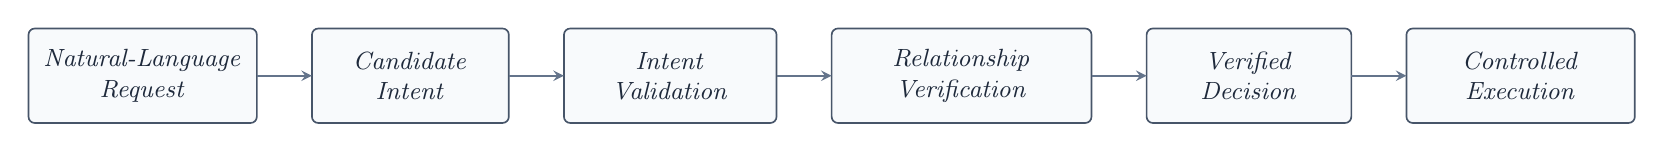
\begin{tikzpicture}[x=1cm,y=1cm,>=stealth]

% ------------------------------------------------------------
% Colours — neutral / non-colorful
% ------------------------------------------------------------
\definecolor{stepfill}{HTML}{F8FAFC}
\definecolor{stepborder}{HTML}{475569}
\definecolor{arrowcol}{HTML}{64748B}
\definecolor{steptext}{HTML}{1E293B}

% ------------------------------------------------------------
% Step 1 — Natural-Language Request
% ------------------------------------------------------------
\draw[
    rounded corners=0.08cm,
    draw=stepborder,
    fill=stepfill,
    line width=0.6pt
]
(0,0) rectangle (2.9,1.2);

\node[
    align=center,
    text=steptext,
    font=\small
] at (1.45,0.6)
{
    \textit{Natural-Language}\\
    \textit{Request}
};

% ------------------------------------------------------------
% Step 2 — Candidate Intent
% ------------------------------------------------------------
\draw[
    rounded corners=0.08cm,
    draw=stepborder,
    fill=stepfill,
    line width=0.6pt
]
(3.6,0) rectangle (6.1,1.2);

\node[
    align=center,
    text=steptext,
    font=\small
] at (4.85,0.6)
{
    \textit{Candidate}\\
    \textit{Intent}
};

% ------------------------------------------------------------
% Step 3 — Intent Validation
% ------------------------------------------------------------
\draw[
    rounded corners=0.08cm,
    draw=stepborder,
    fill=stepfill,
    line width=0.6pt
]
(6.8,0) rectangle (9.5,1.2);

\node[
    align=center,
    text=steptext,
    font=\small
] at (8.15,0.6)
{
    \textit{Intent}\\
    \textit{Validation}
};

% ------------------------------------------------------------
% Step 4 — Relationship Verification
% ------------------------------------------------------------
\draw[
    rounded corners=0.08cm,
    draw=stepborder,
    fill=stepfill,
    line width=0.6pt
]
(10.2,0) rectangle (13.5,1.2);

\node[
    align=center,
    text=steptext,
    font=\small
] at (11.85,0.6)
{
    \textit{Relationship}\\
    \textit{Verification}
};

% ------------------------------------------------------------
% Step 5 — Verified Decision
% ------------------------------------------------------------
\draw[
    rounded corners=0.08cm,
    draw=stepborder,
    fill=stepfill,
    line width=0.6pt
]
(14.2,0) rectangle (16.8,1.2);

\node[
    align=center,
    text=steptext,
    font=\small
] at (15.5,0.6)
{
    \textit{Verified}\\
    \textit{Decision}
};

% ------------------------------------------------------------
% Step 6 — Controlled Execution
% ------------------------------------------------------------
\draw[
    rounded corners=0.08cm,
    draw=stepborder,
    fill=stepfill,
    line width=0.6pt
]
(17.5,0) rectangle (20.4,1.2);

\node[
    align=center,
    text=steptext,
    font=\small
] at (18.95,0.6)
{
    \textit{Controlled}\\
    \textit{Execution}
};

% ------------------------------------------------------------
% Arrows
% ------------------------------------------------------------
\draw[->, line width=0.7pt, draw=arrowcol] (2.9,0.6) -- (3.6,0.6);
\draw[->, line width=0.7pt, draw=arrowcol] (6.1,0.6) -- (6.8,0.6);
\draw[->, line width=0.7pt, draw=arrowcol] (9.5,0.6) -- (10.2,0.6);
\draw[->, line width=0.7pt, draw=arrowcol] (13.5,0.6) -- (14.2,0.6);
\draw[->, line width=0.7pt, draw=arrowcol] (16.8,0.6) -- (17.5,0.6);

\end{tikzpicture}%
}

\caption{Summary of the conceptual workflow of the proposed system.}
\label{fig:concept_summary_flow}
\end{figure}

The following chapter describes how these conceptual elements are realized in
the prototype implementation.